% IEEE BigData 2026 workshop paper (4th Int. Workshop on Trustworthy and Aligned AI), 10 pages including references.
% Protocol frozen 2026-11-12 02:16 CST (hash 22d4f2fa...); registered on OSF (osf.io/bn6va).
\documentclass[conference]{IEEEtran}
\IEEEoverridecommandlockouts
\usepackage{iftex}
\ifXeTeX % Tectonic/XeLaTeX build: use a Times clone so the layout matches pdfLaTeX + IEEEtran
  \usepackage{fontspec}
  \setmainfont{texgyretermes}[Extension=.otf, UprightFont=*-regular, BoldFont=*-bold,
    ItalicFont=*-italic, BoldItalicFont=*-bolditalic]
\fi
\usepackage{cite}
\usepackage{amsmath,amssymb}
\usepackage{graphicx}
\usepackage{booktabs}
\usepackage{array}
\usepackage{multirow}
\usepackage{xcolor}
\usepackage{url}
\usepackage[hidelinks]{hyperref}

\newcommand{\vcr}{\mathrm{VCR}}
\newcommand{\sys}[1]{\textsf{#1}}

\begin{document}

\title{Available Is Not Enforced: A Resource-Matched\\ Benchmark of Verification in Agentic Data Mining}

\author{\IEEEauthorblockN{Ahsan Shahid, Mohammed Muzakkiruddin Ahmed, Hadi Rashid, Abdelrahman Elfikky, and John R. Talburt}
\IEEEauthorblockA{\textit{Department of Computer Science, University of Arkansas at Little Rock}, Little Rock, AR, USA\\
\{axshahid, mmohammed6, harashid, aelfikky1, jrtalburt\}@ualr.edu}}

\maketitle

\begin{abstract}
A data-mining workflow can score well while loading a tampered source, dropping records, or mis-converting units.
We ask whether LLM agents check such properties when a verifying operation is available, and what enforcing checks
changes. Our benchmark has 36 classification and regression tasks from six dataset families with declared and
undeclared defects, a hidden corruption ledger, an oracle verified on every undeclared-defect instance, and an
independent evaluator that scores verified completion without LLM or human judgment. Seven systems (a deterministic
workflow, a single agent, and a three-role team, with and without quality and provenance checks) share data tools
and budgets, and all can use the same hash-verifying load. In 8,352 runs under a protocol frozen before the
evaluation runs, the ungated single agent and team used that load on a content-drift defect in 1 and 12 of 108 runs,
about as often as without the defect, against 104--107 of 108 when the check was enforced with feedback. The primary
contrast, fully gated versus ungated team, was $+0.1$ points (95\% CI $-11.1$ to $+9.9$): content drift contributed
$+7.4$, and two of 18 family--repetition blocks, where a range predicate rejected correct data and no quality-gated
system verified any run, contributed $-8.3$. Without content drift, neither gate's main effect was distinguishable
from zero. A second model from another vendor showed the same uptake pattern. For these models and this tool
description, a verifying operation that is merely available is rarely used, and an enforced check is only as good
as its predicate.
\end{abstract}

\begin{IEEEkeywords}
data mining, data quality, data provenance, benchmark, verification, LLM agents, multi-agent systems
\end{IEEEkeywords}

% =====================================================================
\section{Introduction}
% =====================================================================
Benchmarks for LLM data-science agents report that agents solve a minority of realistic tasks: the best agent in
DSBench solved 34.12\% of its data-analysis tasks~\cite{jing2025dsbench}, the best on the hard tasks of DABstep
reached 14.55\%~\cite{egg2025dabstep}, and the best on the Data Agent Benchmark reached 57\% pass@1 over fragmented
enterprise data~\cite{ma2026dab}. These results measure whether an agent reaches the right answer. For data mining,
a second question matters as much: whether the submitted workflow used the authorised data, kept every record exactly
once, converted units correctly, and fitted learned transforms only on training data. A model can score well while
violating any of these, and leakage of this kind has caused widespread reproducibility failures in applied machine
learning~\cite{kapoor2023leakage}.

Two mechanisms are commonly proposed to make agents more reliable. One is verification: DS-STAR adds an LLM
verifier~\cite{nam2025dsstar}, and DataGovBench reports gains from a planner--executor--evaluator agent with
sandboxed feedback~\cite{liu2025datagovbench}. LLMs are unreliable at correcting themselves without external
feedback~\cite{huang2024selfcorrect}, while tool feedback helps~\cite{gou2024critic}, which suggests checks that are
executed rather than judged. The other is coordination among role-specialised agents~\cite{wu2023autogen,
hong2024metagpt}; controlled studies find that multi-agent structure rarely beats a single agent once computation is
matched~\cite{tran2026single,fu2026moreagents,dylan2026equalcost}.

Recent studies in other domains report that agents often skip an available verification path and that enforced
checks help more than instructions~\cite{zhang2026rite,zhang2026rethinking,sharma2026contextcov}. For data quality,
a metadata-aware gate recovered losses that model capability did not, in a setting where the defect signal never
reached the agent~\cite{besanson2026sarcdq}. We study a nearby case that matters for data mining: the defect leaves
no visible trace in the data, a documented operation available to every system would reveal it, and nothing forces
the agent to use it. Gated systems additionally receive verdicts and two check tools, and a failing check blocks
submission, so ``enforced'' here means enforcement with feedback; we do not separate the two. System names encode
planning and checks: \sys{F} is a deterministic workflow, \sys{S} a single agent, and \sys{M} a three-role team,
followed by \sys{Q} (quality gate), \sys{P} (provenance gate), or \sys{0} (no gates) (Table~\ref{tab:systems}).

The development pilots changed the design before the freeze. Every Tier~1 defect is declared in the task contract
with its remedy, and on these defects all seven systems, including the deterministic workflow, completed 95--100\%
of runs (Section~\ref{sec:pilot}). A benchmark of declared defects alone therefore cannot detect the effect it was
built to measure, so we added Tier~2 defects that violate a stated requirement but lie outside the declared
specification, with severities calibrated by a rule fixed in advance.

\textbf{Contributions.} Based on their published descriptions, none of the closest studies
(Table~\ref{tab:position}) combines the following.
(1)~A data-mining benchmark of 36 tasks with declared and undeclared defects, a hidden corruption ledger, an oracle
checked on every Tier~2 instance, and an independent evaluator of source authority, record coverage, units, and fit
scope rather than final answers (Section~\ref{sec:bench}).
(2)~A budget-matched design that separates planning (deterministic, single agent, three-role team) from quality and
provenance gates, with a full $2\times2$ gate factorial in the team and the hash-verifying operation documented
identically to every system, so that verification that is \emph{available} can be told apart from verification
that is \emph{enforced} (Section~\ref{sec:systems}).
(3)~A protocol frozen and hashed before any evaluation-task run, with a severity calibration rule, a resource-limit
rule, sensitivity analyses, and a second-backbone replication, registered on OSF (Section~\ref{sec:protocol}).
(4)~Pilot evidence that declared-defect benchmarks saturate even for a workflow without an LLM, and that agents
rarely used a documented hash-verifying operation unless provenance checks were enforced (Section~\ref{sec:pilot}).
(5)~Confirmatory evidence (Section~\ref{sec:results}): the ungated single agent and team used the verifying
operation at about the same rate with and without the defect; enforced checking with feedback recovered the defect;
the primary hypothesis was not supported; and one enforced range predicate with false alarms removed every
quality-gated system's completions in two blocks.

% =====================================================================
\section{Related Work}
\label{sec:related}
% =====================================================================
\textbf{Data-science and data agents.}
DSBench~\cite{jing2025dsbench}, MLE-bench~\cite{chan2025mlebench}, InfiAgent-DABench~\cite{hu2024infiagent},
DABstep~\cite{egg2025dabstep}, Spider~2.0~\cite{lei2025spider2}, and DAB~\cite{ma2026dab} score final answers,
predictive scores, or query results; systems such as DS-Agent~\cite{guo2024dsagent}, Data
Interpreter~\cite{hong2024datainterpreter}, and DS-STAR~\cite{nam2025dsstar} add planning and LLM verification.
Auditing agentic data-science solutions across 220 tasks, Li et~al.\ find that most contain at least one
methodological failure such as leakage or inappropriate validation~\cite{li2026silent}. We score explicit
data-handling predicates and hold tasks and tools fixed to compare mechanisms rather than to rank agents.

\textbf{Data governance and cleaning with agents.}
DataGovBench reports that current models lack reliable error correction on 150 governance
tasks~\cite{liu2025datagovbench}. In reference-free agentic data cleaning, a deterministic profiling baseline achieved
the best detection F1 among seven configurations~\cite{fadlallah2026cleaning}. For multi-agent cleaning, debate
improved error detection only with a critic grounded in code execution~\cite{parmar2026debate}, and Fadlallah
et~al.\ vet agent-generated validation rules before execution~\cite{fadlallah2026dqa}. Our gates are fixed,
task-independent predicates, and, like~\cite{fadlallah2026cleaning}, we report a strong deterministic baseline as a
substantive answer rather than a foil.

\textbf{Matched-compute comparisons.}
Single agents match or beat multi-agent systems at equal thinking-token budgets~\cite{tran2026single}; one of six
multi-agent workflows exceeded a single-agent reference across ten benchmarks~\cite{fu2026moreagents}; an evolved
team showed no advantage at fixed model calls~\cite{dylan2026equalcost}; automatically generated multi-agent systems
underperformed self-consistency at up to ten times the cost~\cite{jwalapuram2026illusion}; and across 260
configurations the effect of coordination ranged from $+80.8\%$ to $-70.0\%$ with task structure~\cite{kim2025scaling}.
A taxonomy of over 1,600 multi-agent traces lists task verification among the main failure
groups~\cite{cemri2025mas}. We extend this line to data mining and add whether executable checks are enforced.

\textbf{Available versus enforced verification.}
SARC-DQ found that an agent turned an injected metadata-borne defect into a costly action about 60\% of the time
across four model tiers, while a metadata-aware pre-action gate recovered the loss on the signals its predicates
covered~\cite{besanson2026sarcdq}. LIMBO found that instructed frontier models almost never duplicated a side effect
when a read-back could reveal it~\cite{li2026limbo}. RITE identified recognition of a silent tool error, use of an
available verification path, and integration of its evidence as successive bottlenecks~\cite{zhang2026rite}.
Across seven coding models, completion gates gave larger but costlier gains than instructions, and independent review
the best accuracy--cost trade-off~\cite{zhang2026rethinking}; we do not test an independent-review arm. Executable
guardrails compiled from instruction files raised constraint compliance on SWE-bench Lite from 67.0\% to
88.3\%~\cite{sharma2026contextcov}, verification prompts reduced adoption of corrupted tool
returns~\cite{yang2026overreliance}, and edited tool descriptions received over ten times the usage of the
originals~\cite{faghih2025toolprefs}. When several pre-action gates are composed, a remediation by one gate can invalidate another gate's earlier
judgment~\cite{besanson2026onegate}, which bears on our Q$\times$P interaction. Table~\ref{tab:position} summarises
how our setting differs.

\begin{table}[t]
\caption{Closest related work (summarised from each published abstract)}
\label{tab:position}
\centering\footnotesize\setlength{\tabcolsep}{3pt}
\begin{tabular}{@{}>{\raggedright\arraybackslash}p{0.24\columnwidth}>{\raggedright\arraybackslash}p{0.72\columnwidth}@{}}
\toprule
Work (domain) & What is compared \\
\midrule
SARC-DQ~\cite{besanson2026sarcdq} (data quality) & Model tiers vs.\ a metadata-aware gate; defect signal never in the agent's context \\
LIMBO~\cite{li2026limbo} (side-effecting tools) & Models, harnesses, tool contracts; whether a read-back reveals the outcome \\
RITE~\cite{zhang2026rite} (e-commerce tools) & Silent tool errors; use of an available verification path \\
Rethinking Verification~\cite{zhang2026rethinking} (coding) & Instructions, reminders, completion gates, independent review \\
ContextCov~\cite{sharma2026contextcov} (software eng.) & Prompt-only vs.\ executable guardrails \\
\midrule
\textbf{This study} (data mining) & Deterministic, single-agent, and team systems with and without quality and
provenance gates; verifying operation documented to all; declared vs.\ undeclared defects with an oracle; independent
evaluator; matched budgets; paired instances; frozen protocol \\
\bottomrule
\end{tabular}
\end{table}

\textbf{Data validation, provenance, and benchmark rigor.}
Production ML validates data before training and serving~\cite{polyzotis2019datavalidation,schelter2018deequ}, data
dependencies are a recognised source of technical debt~\cite{sculley2015debt}, mlinspect inspects pipelines for
distribution issues introduced by joins and filters~\cite{grafberger2021mlinspect}, and data cleaning has a long
history~\cite{rekatsinas2017holoclean}. Provenance models represent sources as entities and transformations as
activities~\cite{w3c2013provdm}, and Vamsa infers provenance from data-science scripts~\cite{namaki2020vamsa}. We use
these ideas as treatments that an agent does or does not receive. SWE-bench established execution-based scoring of
agent output~\cite{jimenez2024swebench}, and the Agentic Benchmark Checklist recommends verifying that each task is
solvable and shipping an oracle solver~\cite{zhu2025abc}; items with pass probability near 0.5 are the most
informative~\cite{wang2026dbe}, which motivates our calibration rule.

% =====================================================================
\section{Research Questions and Hypotheses}
\label{sec:rq}
% =====================================================================
Table~\ref{tab:rq} lists the questions. H1 is the only primary hypothesis. The Q and P main effects, the Q$\times$P
interaction, \sys{MQP}$-$\sys{SQP}, and \sys{MQP}$-$\sys{F} on Tier~1 form the secondary family with Holm
adjustment~\cite{holm1979}. \sys{MQP}$-$\sys{F} is restricted to Tier~1 because \sys{F} abstains on every Tier~2
instance by construction. No directional advantage is assumed for coordination (H3) or for agents over the
deterministic baseline (H4).

\begin{table}[t]
\caption{Research questions and prespecified comparisons}
\label{tab:rq}
\centering\footnotesize
\begin{tabular}{@{}p{0.07\columnwidth}p{0.57\columnwidth}p{0.27\columnwidth}@{}}
\toprule
ID & Question / hypothesis & Comparison \\
\midrule
RQ1 & H1: \sys{MQP} has a higher verified-completion rate than \sys{M0} on recoverable tasks (primary) & \sys{MQP} vs \sys{M0} \\
RQ2 & H2: each gate changes the failures it checks; main effects and interaction & \sys{M0}, \sys{MQ}, \sys{MP}, \sys{MQP} \\
RQ3 & H3: coordination vs.\ single agent at equal resources (two-sided) & \sys{MQP} vs \sys{SQP} \\
RQ4 & H4: agents vs.\ deterministic automation (two-sided) & \sys{MQP} vs \sys{F}, Tier~1 \\
RQ5 & Defect type and severity; cost per verified completion & all, by condition \\
RQ6 & Correct refusal on unsatisfiable tasks & all, negative controls \\
RQ7 & Stability with a second LLM vendor & \sys{M0}, \sys{SQP}, \sys{MQP} \\
\bottomrule
\end{tabular}
\end{table}

\textbf{Outcome and estimand.} For a recoverable run $i$, $V_i=1$ if and only if every mandatory external predicate
passes (Section~\ref{sec:evaluator}); abstentions, budget exhaustion, and errors count as $V_i=0$, and
$\vcr=\sum_i V_i/n$. For family $f$ and repetition $r$, let $D_{fr}$ be the mean paired difference
$V_{\sys{MQP}}-V_{\sys{M0}}$ over the family's templates and conditions. The primary estimand
$\Delta=\frac{1}{6}\sum_f\frac{1}{R}\sum_r D_{fr}$ weights each family equally; inference is conditional on the
benchmark portfolio and its defect generators.

\textbf{Prespecified secondary outcome: available versus enforced verification.} For each system we report how often
the trusted traces show the content-verifying load policy (\texttt{authoritative\_verified}) on the content-drift
defect X4, where it is available to every system but enforced only by provenance gates, and on Tier~1, where it is
not needed because the declared authoritative policy suffices (a false-alarm measure). This outcome was fixed before the freeze but after the development pilots.

% =====================================================================
\section{Benchmark}
\label{sec:bench}
% =====================================================================
\textbf{Dataset families.} Table~\ref{tab:data} lists the six families. The public datasets are non-personal UCI
datasets under CC~BY~4.0; AI4I~2020 is itself synthetic~\cite{matzka2020ai4i}, and the Energy Efficiency data
describe simulated buildings~\cite{tsanas2012energy}. D5 and D6 are relational datasets from seeded generators
(NumPy PCG64 substreams derived from SHA-256 of a namespaced string). Twelve smaller development tasks (D5 and D6,
all six templates, a separate namespace) are used only for pilots. Splits are made on canonical records before any
corruption, by groups (identical predictor rows, mixtures, base geometries, machines, batches) or by original order
for AI4I.

\begin{table}[t]
\caption{Dataset families}
\label{tab:data}
\centering\footnotesize\setlength{\tabcolsep}{4pt}
\begin{tabular}{@{}llrl@{}}
\toprule
ID & Source & Rows & Target \\
\midrule
D1 & AI4I 2020~\cite{uci601ai4i} & 10,000 & failure (binary) \\
D2 & Steel Plates Faults~\cite{uci198steel} & 1,941 & fault (7 classes) \\
D3 & Concrete Strength~\cite{uci165concrete,yeh1998concrete} & 1,030 & strength (regression) \\
D4 & Energy Efficiency~\cite{uci242energy} & 768 & heating load (regr.) \\
D5 & Synthetic machinery & 10,000 & failure (binary) \\
D6 & Synthetic process & 9,000 & output (regression) \\
\bottomrule
\end{tabular}
\end{table}

\textbf{Templates and contracts.} Six templates per family give 36 tasks: T1 single-source modeling; T2 two-table
reconstruction by a canonical key; T3 three-table integration; T4 harmonisation of documented affine shard
representations; T5 version-aware source selection against an authoritative as-of catalog; and T6 per-observation
aggregates (mean, population standard deviation, count) from child readings. Each table has 20 logical shards per
partition. Every system receives the same machine-readable contract and natural-language rendering (target,
permitted and excluded predictors, source versions, keys, units, aggregation rules, missing-value policy, value
ranges, output schema, budget). The contract never reveals corrupted locations, hidden labels, or defect counts.

\textbf{Tier 1: declared defects.} A clean condition C0 and six corruptions: C1/C2 affect 5\%/20\% of numeric cells
(half missing, half encoded as strings in a documented grammar); C3/C4 affect 5\%/20\% of observation keys (exact
duplicates or aliases listed in a supplied catalog); C5/C6 affect 1/4 of shards (a documented representation change
or a stale source that fails the authoritative version and hash). Each defect and its remedy are declared.

\textbf{Tier 2: defects outside the declared specification.} Tier~2 defects violate a requirement the contract
already states, are detectable by an existing check or by inspecting the data, and are repairable by a general
operation documented identically to every system in both tiers (Table~\ref{tab:tier2}). The format specification
does not describe them, so \sys{F}, whose rules are written from it, does not repair them by design.
\emph{X2 key variants:} keys in lower case, without zero padding, or with spaces, not in the alias table.
\emph{X3 undeclared representation:} some shards use a catalogued representation not declared for that shard, so
values fall outside the contract ranges; only choices with a unique in-range repair are used.
\emph{X4 content drift:} for $k$ shards, the primary authorised file no longer matches the authorised SHA-256 while
its catalog entry still declares it; a replica with the authorised content exists but has an earlier modification
time, so neither ``latest modified'' nor ``latest snapshot'' selects it. Drifted values stay inside the value ranges
and are independent of labels, so quality checks rarely flag X4 (on the evaluation tasks the range check fired on
drifted data only in T4, whose shards are stored in an affine representation). To avoid revealing which defect is present, every
Tier~2 instance carries an ingest-batch column, a replica of each observation-grain table, and published value
ranges. A near-duplicate defect (X1) was dropped before the freeze because no provenance check could detect it and
both baseline agents completed every X1 pilot run.

\begin{table}[t]
\caption{Tier~2 defects. Levels a/b/c; frozen level in bold.}
\label{tab:tier2}
\centering\footnotesize\setlength{\tabcolsep}{3pt}
\begin{tabular}{@{}lp{0.27\columnwidth}p{0.25\columnwidth}l@{}}
\toprule
ID & Levels & Detected by & Repair \\
\midrule
X2 & 5\% / \textbf{10\%} / 20\% of keys & record coverage, label match (Q) & \texttt{\scriptsize normalize\_key} \\
X3 & \textbf{1} / 2 / 4 of 20 shards & value ranges (Q) & \texttt{\scriptsize infer\_representation} \\
X4 & 1 / \textbf{2} / 4 of 20 shards & content hash (P) & \texttt{\scriptsize authoritative\_verified} \\
\bottomrule
\end{tabular}
\end{table}

\subsection{Hidden ledger, evaluator, and solvability}
\label{sec:evaluator}
The generator records every injected change (location, type, before and after values or hashes, severity
denominator, seed) outside the agent environment. Hidden test corruption is applied by the evaluator, which runs in a
separate process, is the only component with hidden labels and the ledger, and does not call the internal gates.
$V_i=1$ requires that: the required artifacts and a permitted estimator exist; target, source authority, and feature
exclusions are correct; records, join granularity, unit conversions, and aggregates match an independent reference
(absolute tolerance $10^{-8}$, relative $10^{-6}$); learned preprocessing was fitted on training data only; the
frozen workflow returns one finite prediction per hidden test record with valid probabilities; artifact hashes are
consistent; and the run stayed within its limits. At hidden evaluation only the frozen declarative graph and fitted
estimator run, with no LLM calls or refitting. Known-correct, valid-alternative, and known-incorrect fixtures (wrong
join, duplicated predictions, wrong version, unit mismatch, bad aggregate, forbidden predictor, changed hash,
invalid probabilities) must produce their expected verdicts before any agent run. An oracle solver, which adds the
general Tier~2 repairs to the declarative workflow, reproduced the hidden reference on all 216 development Tier~2
instances, and at the freeze on all $36\times3\times3=324$ formal Tier~2 instances; the freeze is written only if
this check passes~\cite{zhu2025abc}.

% =====================================================================
\section{Systems}
\label{sec:systems}
% =====================================================================
\begin{table}[t]
\caption{System key. All systems share the data tools, candidate models, and budgets; gated systems also have the two check tools.}
\label{tab:systems}
\centering\footnotesize\setlength{\tabcolsep}{5pt}
\begin{tabular}{@{}lllcc@{}}
\toprule
System & Planning & LLM & Quality gate & Provenance gate \\
\midrule
\sys{F}   & deterministic workflow & no  & yes & yes \\
\sys{S0}  & single agent           & yes & --  & -- \\
\sys{SQP} & single agent           & yes & yes & yes \\
\sys{M0}  & three-role team        & yes & --  & -- \\
\sys{MQ}  & three-role team        & yes & yes & -- \\
\sys{MP}  & three-role team        & yes & --  & yes \\
\sys{MQP} & three-role team        & yes & yes & yes \\
\bottomrule
\end{tabular}
\end{table}

\textbf{Shared tools.} All systems act only through the same bounded tools: \texttt{list\_sources},
\texttt{inspect\_schema}, \texttt{profile\_data}, \texttt{query\_data} (read-only SQL on in-memory
DuckDB~\cite{raasveldt2019duckdb}), \texttt{materialize\_features} (a validated declarative graph of
\texttt{load}, \texttt{parse\_numeric}, \texttt{to\_canonical}, \texttt{map\_alias}, \texttt{normalize\_key},
\texttt{infer\_representation}, \texttt{dedupe}, \texttt{join}, \texttt{aggregate}, \texttt{drop\_missing\_rows},
\texttt{project}), \texttt{fit\_evaluate} (at most six candidate evaluations), \texttt{submit}, and \texttt{abstain}
with a structured reason. Gated systems can also call \texttt{quality\_check} and \texttt{provenance\_check}. Trusted
wrappers, not model statements, record source handles, row counts, hashes, and fit partitions for every system. The
six candidate models per task type are fixed scikit-learn~\cite{pedregosa2011sklearn} pipelines (two regularised
linear models, two random forests, two histogram gradient boosting models) with preprocessing fitted on training
folds only.

\textbf{Quality gate (Q).} After each materialisation and at submission: required columns only; excluded predictors
absent; numeric types; key uniqueness; record coverage against the partition manifest; contract value ranges;
aggregate counts and non-negative standard deviations; conversion of declared shard representations; no dropped
rows. After each fit: every training row matches a label and validation coverage is complete.
\textbf{Provenance gate (P).} For every loaded table: an unambiguous authority record; authorised version and
declared hash for every shard; no authorised shard absent; recomputed content hash equals the authorised hash; source
lineage for every required column; fits used only the training partition; the submitted artifact was produced and
evaluated in this run. Gate verdicts are returned with the failing checks; a failing gate at submission blocks it,
leaving at most two repair cycles or abstention. Ungated systems receive ordinary tool output and errors only.

\textbf{The seven systems.} \sys{F} is a deterministic contract-driven workflow without an LLM: it loads
authoritative sources, parses declared representations, maps declared aliases, removes exact duplicates, performs
declared joins and aggregates, runs both gates, evaluates all six candidates, and submits, or abstains if a gate
fails. Its rules come from the declared specification and the development tasks, and it never branches on a task
identifier. \sys{S0} and \sys{SQP} are a single agent without and with both gates. \sys{M0}, \sys{MQ}, \sys{MP}, and
\sys{MQP} are a three-role team (coordinator, data manager, mining agent) without gates, with Q, with P, and with
both. Roles share the backbone, tools, and a structured blackboard; only the coordinator can submit, and every role's
tokens and calls are charged to one run budget.

% =====================================================================
\section{Protocol}
\label{sec:protocol}
% =====================================================================
\textbf{Models.} Backbone A is \texttt{Qwen/Qwen3.8-27B}~\cite{qwen2026qwen38} (27.8B parameters) and backbone B
\texttt{google/gemma-4-31B-it}~\cite{google2026gemma4} (31.3B), both Apache-2.0, pinned to immutable revisions, and
served in BF16 with vLLM~0.33.0~\cite{kwon2023vllm} on one 96\,GB NVIDIA RTX PRO 6000 Blackwell. Both use
temperature 0.2, top-$p$ 0.9, top-$k$ 40, a 16,384-token context, 1,024 output tokens per call, reasoning mode
disabled, and schema-constrained JSON actions, so results describe non-reasoning use.

\textbf{Resource limits.} Per run: 48 model calls across all roles, 40 tool calls, six candidate evaluations, two
repair cycles, and 600\,s of active time. The token limit follows a rule fixed before the pilots,
$\max(\text{protocol limit},\lceil1.25\,p_{95}\rceil)$ of pilot usage capped at the 300,000-token pilot limit. On the
1,377 backbone-A pilot runs in the frozen conditions that ended in submission or abstention, $p_{95}=245{,}962$
(median 141,224), so the limit is the cap, 300,000 tokens. Because every call re-sends the growing context, this
admits roughly 30 single-agent or 40--45 team calls; it binds on Tier~2, and we make no claim about larger budgets.

\textbf{Pilots and calibration.} All pilots use the development tasks only: E0 (C0, C6; 336 runs), E0S (C1--C5; 840),
E0SB (C0--C6, backbone B; 504), E0X (X1--X3; 741 of 756), and the calibration pilot E0X2 (X2--X4 at three levels,
two repetitions; 1,512). The rule, fixed before E0X, selects for each defect the level whose pooled \sys{S0}+\sys{M0}
VCR is closest to 0.5 (ties to the lower level). It selected X2b (0.750, tied with X2c), X3a (0.708), and X4b
(0.083); the target of 0.5 was not reachable, and we did not re-tune.

\textbf{Formal experiments.} E1 runs all seven systems with backbone A on the 36 evaluation tasks, ten recoverable
conditions (C0--C6, X2b, X3a, X4b), and three paired repetitions: 7,560 runs. E2 (gate factorial) and E3 (condition
and cost) reuse E1. E4 replicates \sys{M0}, \sys{SQP}, and \sys{MQP} with backbone B on six tasks fixed in advance
(D1-T5, D2-T2, D3-T4, D4-T6, D5-T3, D6-T1) under the same conditions: 540 runs. E5 runs all seven systems on the same
six tasks with two unsatisfiable variants, an absent required version (N1) and conflicting authority records without
precedence (N2): 252 runs; correct refusal requires no predictions and the matching structured reason. E6 replays
frozen submissions under invariance checks (row and column order, equivalent numeric representations) and corruption
checks (wrong version, missing prediction, changed hash). Run order is randomised within paired blocks and agent
state is reset before every run. A verified infrastructure failure may be retried once; agent failures are never
retried. Each run is stored as its own record, so an interrupted session resumes only runs without a record, and
every session first verifies the freeze manifest and the content digest of every task instance. Eight runs execute
concurrently against one vLLM server, so active time includes waiting for the shared server.

\textbf{Freeze and registration.} The protocol was frozen on 12 Nov.\ 2026 at 02:16 CST, before any evaluation-task
run. The manifest records the protocol hash (\texttt{22d4f2fa\ldots}), the code hash, the model lock, the dataset,
split, and canonical-data manifest hashes, the limits, three repetitions, the frozen Tier~2 levels, and the analysis
plan below. The frozen package was registered on OSF (\url{https://osf.io/bn6va}; embargoed until publication) on
13 Nov.\ (UTC), while the formal runs were in progress and before any formal result was analysed. All changes from
the first written protocol (30 Oct.\ 2026) were made before the freeze (Table~\ref{tab:deviations}).

\begin{table}[t]
\caption{Changes from the first written protocol, all before the freeze}
\label{tab:deviations}
\centering\footnotesize\setlength{\tabcolsep}{3pt}
\begin{tabular}{@{}p{0.27\columnwidth}p{0.3\columnwidth}p{0.37\columnwidth}@{}}
\toprule
Item & First protocol & Frozen \\
\midrule
Backbones & Qwen3-Coder-30B-A3B; Qwen2.5-Coder-14B & Qwen3.8-27B; Gemma-4-31B-it \\
Token limit & 30,000 & 300,000 (prespecified pilot rule) \\
Defects & C0--C6 & C0--C6 plus X2b, X3a, X4b \\
Formal runs & 5,922 & 8,352 \\
Primary analysis & all core tasks & Tier~1 and Tier~2 pooled, plus per-tier and no-X4 \\
\sys{MQP}$-$\sys{F} (Holm) & all tasks & Tier~1 only \\
Added outcomes & -- & verifying-operation uptake; budget-exhaustion composition \\
Isolation & containers & process-level \\
\bottomrule
\end{tabular}
\end{table}

\textbf{Analysis plan.} Uncertainty for $\Delta$ uses a paired block bootstrap with 10,000 draws that keeps the six
families fixed and resamples repetition blocks within each family, carrying all templates, conditions, and systems
together~\cite{efron1979bootstrap,saravanan2020hierarchical}. Gate effects are estimated on the probability scale:
$Q=\tfrac12[(V_{\sys{MQ}}-V_{\sys{M0}})+(V_{\sys{MQP}}-V_{\sys{MP}})]$,
$P=\tfrac12[(V_{\sys{MP}}-V_{\sys{M0}})+(V_{\sys{MQP}}-V_{\sys{MQ}})]$, and
$Q\!\times\!P=V_{\sys{MQP}}-V_{\sys{MQ}}-V_{\sys{MP}}+V_{\sys{M0}}$. Because pooling the tiers in H1 was decided after
the calibration pilots, we prespecified, without Holm adjustment, every contrast on each tier, the Tier~2 minus
Tier~1 difference, and analyses excluding X4. Three repetition blocks give only ten distinct resamples per family,
so we also prespecified (a)~a mixed-effects logistic regression of $V$ on system with random intercepts for task
and family--repetition block, (b)~the bootstrap interval with variance inflation $n/(n-1)$, and (c)~per-family and
leave-one-family-out estimates. Predictive metrics (average precision and macro-F1; RMSE and MAE) are reported only
for verified runs. We describe the terminal state and tool-call composition of budget-exhausted runs. The paired sign-flip test
flips the sign of each of the 18 family--repetition block differences at random (10,000 draws, two-sided) and
compares the family-weighted mean with the observed one; Holm adjustment uses these $p$ values. All intervals are
conditional on the 36 tasks. Failure to reject a difference is not evidence of equivalence.

% =====================================================================
\section{Pre-Freeze Pilot Results (Development Tasks)}
\label{sec:pilot}
% =====================================================================
These results come from the 12 development tasks (two synthetic families) and were used to design the frozen
protocol; they are not confirmatory. On Tier~1 (C0--C6, 168 runs per system), \sys{F} verified 168 of 168 runs and
every agentic system 95.8--98.2\%; \sys{MQP}$-$\sys{M0} was $-0.6$ points. Backbone B was also at the ceiling (\sys{M0}
0.964, \sys{SQP} 0.964, \sys{MQP} 0.976). A first backbone-B pilot exposed a tool bug affecting 28 runs; we fixed it and
reran all 504 runs, so that no run was selected by its outcome. In the Tier~2 calibration pilot (72 runs per defect and
system), \sys{F} abstained on all Tier~2 runs, and on X4 \sys{S0} and \sys{M0} used the hash-verifying load in 2 and 5
runs, \sys{MQ} in 22, and the systems with enforced provenance checks in 71--72. On X2, gates did not help (\sys{SQP}
0.736 vs.\ \sys{S0} 0.833): 96 of 102 failed agentic X2 runs ended at the token limit while still exploring (25--28
schema, profiling, and query calls on average, against 8--12 per Tier~1 run), and 61 never fitted a model. Applied to
pilot cells in the frozen conditions, the frozen estimator gave $+9.2$ points for \sys{MQP}$-$\sys{M0} ($-0.6$ on
Tier~1, $+31.9$ on Tier~2); these cells informed the design and do not support H1.

% =====================================================================
\section{Confirmatory Results}
\label{sec:results}
% =====================================================================
All 8,352 scheduled runs were recorded (E1 7,560; E4 540; E5 252). Ten E1 runs were retried once with identical
inputs as verified infrastructure failures: eight were in progress when the JupyterHub server was stopped externally,
and two received a zero generation budget from the serving engine because the prompt filled the context. No run was
retried after an agent failure. Table~\ref{tab:main} gives VCR by system and tier and Table~\ref{tab:contrasts} the
prespecified contrasts. Two E1 and seven E4 runs reached the 600\,s limit; every other budget-exhausted run
reached the token limit.

\begin{table}[t]
\caption{Confirmatory VCR by system and tier (E1, backbone A, 36 tasks, 3 repetitions)}
\label{tab:main}
\centering\footnotesize\setlength{\tabcolsep}{4pt}
\begin{tabular}{@{}lrrrrr@{}}
\toprule
System & Tier 1 & Tier 2 & All & X2, X3 & X4 \\
 & ($n$=756) & ($n$=324) & ($n$=1,080) & ($n$=216) & ($n$=108) \\
\midrule
\sys{F}   & 0.889 & 0.000 & 0.622 & 0.000 & 0.000 \\
\sys{S0}  & 0.958 & 0.429 & 0.799 & 0.639 & 0.009 \\
\sys{M0}  & 0.938 & 0.451 & 0.792 & 0.625 & 0.102 \\
\sys{MQ}  & 0.841 & 0.537 & 0.750 & 0.662 & 0.287 \\
\sys{MP}  & 0.938 & 0.738 & 0.878 & 0.648 & 0.917 \\
\sys{SQP} & 0.858 & 0.747 & 0.825 & 0.704 & 0.833 \\
\sys{MQP} & 0.835 & 0.694 & 0.793 & 0.620 & 0.843 \\
\bottomrule
\end{tabular}
\end{table}

\begin{table*}[t]
\caption{Prespecified contrasts (percentage points, family-weighted, 95\% block-bootstrap interval). Holm-adjusted
sign-flip $p$ for the secondary family on the pooled estimate. ``No X4'': all recoverable conditions except X4.}
\label{tab:contrasts}
\centering\footnotesize\setlength{\tabcolsep}{3pt}
\begin{tabular}{@{}lrrrrrr@{}}
\toprule
Contrast & All (pooled) & Holm $p$ & Tier 1 & Tier 2 & No X4 & Tier 2 $-$ Tier 1 \\
\midrule
H1: \sys{MQP}$-$\sys{M0} (primary) & $+0.1$ [$-11.1$, $+9.9$] & -- & $-10.3$ [$-21.3$, $-0.7$] & $+24.4$ [$+12.3$, $+34.9$] & $-8.1$ [$-19.1$, $+1.4$] & $+34.7$ [$+30.2$, $+38.8$] \\
Q main effect & $-6.3$ [$-17.3$, $+3.8$] & 0.50 & $-10.0$ [$-21.1$, $+0.3$] & $+2.2$ [$-9.0$, $+12.0$] & $-7.7$ [$-18.7$, $+2.4$] & $+12.1$ [$+9.1$, $+15.3$] \\
P main effect & $+6.4$ [$+5.5$, $+7.4$] & $<$0.001 & $-0.3$ [$-1.2$, $+0.5$] & $+22.2$ [$+19.8$, $+24.7$] & $-0.5$ [$-1.4$, $+0.5$] & $+22.6$ [$+19.9$, $+25.2$] \\
Q$\times$P interaction & $-4.4$ [$-6.2$, $-2.5$] & 0.013 & $-0.7$ [$-2.5$, $+1.2$] & $-13.0$ [$-18.5$, $-7.4$] & $-2.0$ [$-3.8$, $-0.2$] & $-12.3$ [$-18.4$, $-6.0$] \\
\sys{MQP}$-$\sys{SQP} & $-3.2$ [$-4.5$, $-1.8$] & 0.041 & $-2.4$ [$-3.8$, $-0.7$] & $-5.2$ [$-8.0$, $-2.5$] & $-3.7$ [$-5.2$, $-2.0$] & $-2.9$ [$-6.3$, $+0.2$] \\
\sys{MQP}$-$\sys{F} (Tier~1) & -- & 0.001 & $-5.4$ [$-7.9$, $-2.5$] & -- & -- & -- \\
\bottomrule
\end{tabular}
\end{table*}

\begin{figure}[t]
\centering
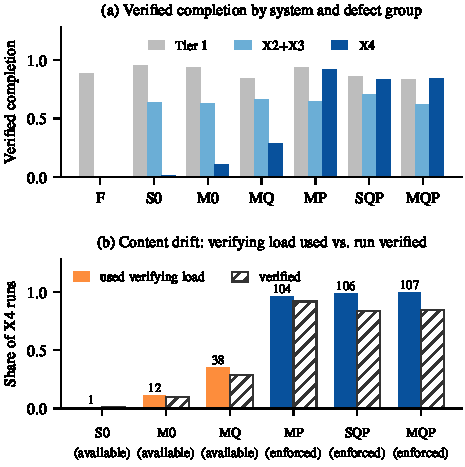
\includegraphics[width=\columnwidth]{figures/fig_main.pdf}
\caption{E1 results (backbone A, 36 evaluation tasks, three repetitions). (a)~Verified completion on declared
defects (Tier~1), undeclared defects other than content drift (X2, X3), and content drift (X4). (b)~On X4, the
share of runs that used the content-verifying load policy, which every system can use, and the share that were
verified; numbers above bars are run counts out of 108.}
\label{fig:main}
\end{figure}

\begin{table}[t]
\caption{Use of the content-verifying load policy (\texttt{authoritative\_verified}) from trusted traces, E1}
\label{tab:verify}
\centering\footnotesize\setlength{\tabcolsep}{4pt}
\begin{tabular}{@{}lccrrr@{}}
\toprule
System & Enforced & \multicolumn{2}{c}{X4 ($n$=108)} & \multicolumn{2}{c}{Tier~1 ($n$=756)} \\
\cmidrule(lr){3-4}\cmidrule(l){5-6}
 & & used & verified & used & rate \\
\midrule
\sys{S0}  & no  & 1   & 1  & 3   & 0.4\% \\
\sys{M0}  & no  & 12  & 11 & 99  & 13.1\% \\
\sys{MQ}  & no  & 38  & 31 & 175 & 23.1\% \\
\sys{MP}  & yes & 104 & 99 & 228 & 30.2\% \\
\sys{SQP} & yes & 106 & 90 & 12  & 1.6\% \\
\sys{MQP} & yes & 107 & 91 & 321 & 42.5\% \\
\bottomrule
\end{tabular}
\end{table}

\textbf{Agents rarely verify unless made to.} On X4 the ungated single agent used the hash-verifying load in 1 of 108
runs and the ungated team in 12; systems whose provenance check was enforced used it in 104--107
(Table~\ref{tab:verify}, Fig.~\ref{fig:main}b). For \sys{S0} and \sys{M0} the use did not respond to the defect:
\sys{M0} used the policy in 11.1\% of X4 runs and in 13.1\% of Tier~1 runs, where nothing had drifted, and \sys{S0} in
0.9\% and 0.4\%. Their most frequent first failure on X4 was a wrong source version (105 and 88 of 108). \sys{MQ},
whose task text mentions quality checks, used the policy more on X4 than on Tier~1 (35.2\% vs.\ 23.1\%); only 2 of
its 38 X4 uses followed a failed range check (both in T4), so the difference is not explained by gate verdicts. On
Tier~1, use was highest on C6, the declared stale-source condition (\sys{M0} 25, \sys{MQ} 37, \sys{MP} 48, \sys{MQP} 75
of 108), where the declared authoritative policy already suffices; this use is harmless. Of the 37 gated X4 runs that
used the policy but were not verified, 32 ended at the budget limit, 21 of them in the false-alarm blocks below. With
backbone B (E4), \sys{M0} used the policy in 0 of 18 X4 runs and 0 of 126 Tier~1 runs, \sys{SQP} in 17 and \sys{MQP} in
18 of 18 X4 runs.

\textbf{Primary hypothesis.} H1 was not supported: \sys{MQP}$-$\sys{M0} was $+0.1$ points ($-11.1$ to $+9.9$; sign-flip
$p=1.0$). The variance-inflated interval was $-13.1$ to $+13.3$ and the leave-one-family-out range $-2.3$ to $+4.4$.
The prespecified mixed-effects logistic model gave an odds ratio of 1.01 (0.86 to 1.19), but it has no
system-by-block term, while the dominant effect here is exactly such an interaction; adding a random system slope per
block (not prespecified) gave 1.30 (1.05 to 1.61), because that model treats the two false-alarm blocks as
block-level deviations. We keep the prespecified block bootstrap as the primary result. The pooled null hides opposite effects: $-10.3$ points on Tier~1 and $+24.4$ on Tier~2, and per family
$+12.2$ (D1), $-21.7$ (D2), $+12.2$ (D3), $-18.3$ (D4), $+10.0$ (D5), and $+6.1$ (D6).

\textbf{A quality-gate false alarm.} The negative D2 and D4 estimates have one cause. The contract publishes
plausible value ranges computed on the training partition and padded by 25\% of the span. In one repetition of D2
and one of D4, some validation-partition values fall outside these ranges, so the quality gate's range check fails on
correct data. In these two blocks (120 runs per system), \sys{F} abstained in every run, as its rule requires, and the
three systems with a quality gate verified none: they could not pass the gate and mostly ran out of budget trying to
repair data that was correct (\sys{MQ} 107, \sys{MQP} 109, \sys{SQP} 97 runs at the token limit). Systems without
the quality gate verified 75.0\% (\sys{M0}), 75.8\% (\sys{S0}), and 86.7\% (\sys{MP}) of the same runs. These blocks
account for all 84 of \sys{F}'s Tier~1 failures. The ranges are published as plausible canonical ranges, not as a
requirement that verified completion depends on: the evaluator scores units and values against the hidden reference,
and the data in these blocks match it. X3 violates the stated units requirement, and the ranges are the evidence by
which it can be detected. The same predicate therefore produced both outcomes: on \sys{F}'s loads it fired on all 108
X3 runs, on correct data in 2 of 18 blocks and nowhere else, and on drifted data in T4. Counting abstentions in the two
blocks as correct, a sensitivity analysis we add here, changes \sys{F}'s Tier~1 VCR to 1.000 but recovers only 8
(\sys{MQ}), 10 (\sys{MQP}), and 18 (\sys{SQP}) of 120 gated runs, because the gated agents mostly kept repairing
rather than abstaining. As a post-hoc analysis that is not part of the protocol, excluding
the two blocks gives Tier~1 VCR of 1.000 for \sys{F} and 0.939--0.966 for every agentic system, and H1 of $+9.3$
points ($+7.0$ to $+11.4$), of which almost all comes from X4: without X4 it is $+0.9$ ($-0.9$ to $+2.8$). D2 and D4
then keep only two blocks each.

\textbf{Without content drift.} Excluding X4 (prespecified), H1 was $-8.1$ points and the P main effect $-0.5$
(Table~\ref{tab:contrasts}). Per defect, \sys{MQP}$-$\sys{M0} was $-8.3$ ($-22.2$ to $+3.7$) on X2, $+7.4$
($-5.6$ to $+19.5$) on X3, and $+74.1$ ($+60.2$ to $+86.1$) on X4, where the P effect was $+68.5$. The one clear
non-X4 gain was the gated single agent on X3 (\sys{SQP}$-$\sys{S0} $+23.1$, $+10.2$ to $+35.2$), where the quality
gate detects out-of-range shards.

\textbf{Gate factorial, coordination, and the deterministic baseline.} After Holm adjustment, the P main effect
($+6.4$), the negative Q$\times$P interaction ($-4.4$), \sys{MQP}$-$\sys{SQP} ($-3.2$), and \sys{MQP}$-$\sys{F} on
Tier~1 ($-5.4$) were significant; the Q main effect ($-6.3$) was not. The negative interaction means that Q and P
gains did not add on Tier~2 ($-13.0$). The team did not beat the single agent at matched budget and took longer
(mean active time 223\,s for \sys{MQP} versus 138\,s for \sys{SQP}; 248k versus 224k tokens per verified completion).
\sys{F} beat the gated team on Tier~1 even with its false-alarm abstentions.

\textbf{Budget, refusal, second backbone, and replay.} Runs that ended at the token limit numbered 198 (\sys{MQP}),
181 (\sys{MQ}), and 156 (\sys{SQP}) of 1,080, against 52 (\sys{S0}), 77 (\sys{M0}), and 76 (\sys{MP}); outside the two
false-alarm blocks the gated counts were 89, 74, and 59. As in the pilots, exhausted runs were still exploring
(19--26 schema, profiling, and query calls on average), and 43--57\% of them never fitted a model. On unsatisfiable
tasks (E5) every system refused correctly in 33--36 of 36 runs; the five false submissions were all on conflicting
authority records (N2). With backbone B (E4), \sys{MQP}$-$\sys{M0} was $0.0$ points ($-12.2$ to $+10.6$): $-15.9$
on Tier~1 and $+37.0$ on Tier~2, and on X4 \sys{M0} verified 0 of 18 runs against 13 for \sys{MQP} and 16 for
\sys{SQP}; in the affected repetitions of D2-T2 and D4-T6 the gated systems verified none of 40 runs and \sys{M0} 17
of 20. The E6 audit replayed 146 retained submissions. All 146 reproduced their recorded outcome and were invariant to
row and column order, and a changed artifact hash was detected in all 137 verified ones. Two corruption checks did not
always return the expected failure code: the wrong-version check (31 of 137) and the missing-record check (14 of 137).
In 18 cases the check applied no corruption, because every numeric column of the C1/C2 instance was string-encoded; in
24 (12 submissions) the workflow used the hash-verifying load, which does not load a file whose content fails its hash
when an intact replica exists; and in 3 the corruption was flagged under a different failure code.

% =====================================================================
\section{Discussion and Threats to Validity}
\label{sec:discussion}
% =====================================================================
\textbf{Available is rarely used.} The clearest result is behavioural. A documented operation that would have
solved the content-drift defect was used by the ungated single agent and team at a background rate that did not
change when the defect was present; they relied on the catalog's declared authority without recomputing content. This
extends to data mining what studies in coding and tool use report~\cite{zhang2026rite,zhang2026rethinking}, and the
second model behaved the same way. X4 gives agents no visible signal, so the informative quantity is this base rate of
unprompted verification, which is conditional on one tool description and on two non-reasoning models; \sys{MQ}'s
higher use suggests that merely mentioning checks raises it.

\textbf{Enforced is only as good as its predicate.} Enforcement recovered most drift runs, but one predicate
with false alarms, a value range estimated on training data, removed every quality-gated system's completions in two
of eighteen blocks, while ungated agents, free to ignore a range that the data did not need to satisfy, completed most of
those runs. A blocking gate turns each false alarm into a failure, and agents spent their budget trying to repair
correct data. Gates for agentic data mining therefore need calibrated predicates and a way to contest a verdict, for
example advisory checks or an evidence-based override. The deterministic workflow, which abstains on any failed
check, behaved the same way. The range predicate shows the trade-off directly: the check that detected every X3
instance also rejected correct data in two blocks. Excluding those blocks (post hoc), declared defects were again near
the ceiling (\sys{F} 1.000, agents 0.939--0.966), and the remaining gate benefit came from content drift.

\textbf{Coordination did not pay.} At matched budgets the gated team was 3.2 points below the gated single agent and
took about 60\% longer, consistent with matched-compute studies in other domains~\cite{tran2026single,dylan2026equalcost}.

\textbf{The false alarm as a protocol finding.} The range predicate was frozen before the evaluation runs, and the
development families did not trigger it; the oracle check at the freeze verified solvability by the evaluator, not
passage of the gates. We report the affected blocks as they ran and give the exclusion only as a labelled post-hoc
analysis. A pre-freeze check that the oracle output passes every gate on every instance would have caught it.

\textbf{Construct validity.} VCR measures compliance with explicit predicates, not universal correctness, and a weak
but properly fitted model can pass; we report predictive metrics beside it. Contracts make the tasks easier than
open-ended discovery; the study concerns bounded, contract-defined automation. Tool use depends on
wording~\cite{faghih2025toolprefs}; all systems see one fixed description of each operation, so the measured uptake
is conditional on that wording.

\textbf{Design of Tier 2 and the role of X4.} Each Tier~2 defect was built to be detectable by a specific check, so a
positive effect of P on X4 is close to a manipulation check and X4 can dominate the pooled H1. We therefore do not
read a large P effect as evidence that provenance gates improve data mining in general; the informative quantities
are the X4-excluded and per-defect estimates and the ungated systems' use of the available operation. Documenting
the repair operations to every system could hint that such defects exist; we document them identically in both tiers
and report their Tier~1 use as a false-alarm measure.

\textbf{Enforcement, feedback, and salience.} Gated systems receive verdicts, two check tools, and a configuration
line in the task text, and a failing check blocks submission. The design estimates enforced checking \emph{with}
feedback and does not separate it from the mention of a check or from an explicit instruction to verify; instructed
and advisory arms would, and are not part of the frozen design. The title's contrast should be read in this sense.

\textbf{Statistical and external validity.} Three repetition blocks per family give unstable intervals, hence the
prespecified sensitivity analyses. Six purposively chosen families do not support population claims, and the 36
tasks are not 36 independent datasets. Two backbones from two vendors, both without reasoning mode, give limited
cross-vendor evidence, and the Tier~2 levels were calibrated on backbone A. Public datasets may appear in training
data. Budgets are matched in total tokens and calls, not effective calls: team roles carry shorter contexts, so the
same limit admits more team calls. Isolation is process-level, not container-based. No human repairs or reruns any
scored run.

\textbf{Deviations after the freeze.} The frozen E6 audit code failed under pandas~3 on integer columns after all
runs were recorded; we ran it with a one-line type conversion, without modifying the frozen package, and the frozen
pipeline then completed and passed its freeze verification. No run, outcome, or analysis setting changed.

% =====================================================================
\section{Reproducibility and Research Ethics}
% =====================================================================
The frozen package (code, prompts, configuration, manifests with SHA-256 checksums, model lock, study plan, analysis
scripts, and a script that recomputes every hash) is registered on OSF; on publication we will release it with the
task generators and seeds (master seed 20261030), the evaluator and fixtures, every run record and trusted trace, and
the scripts that produce every table. Pilot runs are archived separately from confirmatory runs, including the 504
first-E0SB runs. The pilots used 23.4 GPU-hours and the formal experiments about 47.5 (E1 43.0, E4 4.1, E5 0.4), counting
a 14.3-hour E1 session whose accounting record was lost when the server was stopped externally. The study uses no human participants, personal data, human
annotation, or human or LLM grading.

% =====================================================================
\section{Conclusion}
% =====================================================================
We built a data-mining benchmark and a frozen protocol that separate planning, quality checks, and provenance checks
under matched resources, with a verifying operation available to every system but enforced only for some. In 8,352
runs with two open models used without reasoning mode, the ungated agents rarely used the verifying operation,
enforced checking with feedback recovered a defect they otherwise missed, and an enforced range predicate with false
alarms removed the completions of every system that enforced it in the two blocks where it fired; the pooled primary
contrast was null. The gated team did not beat the deterministic workflow on declared defects. Within the limits of
one tool description and two models, the lesson is that a verifying operation that agents may skip is mostly
skipped, and that a blocking check needs a predicate calibrated to what the contract actually requires, or a way for
the agent to contest it; advisory and contestable checks remain to be tested.

\section*{Acknowledgment}
The experiments ran on an NVIDIA RTX PRO 6000 Blackwell GPU that NVIDIA donated to the Department of Computer
Science at UA Little Rock, which now owns and operates it.
The authors used an AI assistant (Kiro, with Anthropic Claude models) to help write the study software and to draft
and edit the text of all sections of this paper. The authors reviewed the generated text, checked every reported
number against the run records and every reference against its source, and take full responsibility for the
content.

\bibliographystyle{IEEEtran}
\bibliography{refs}

\end{document}
